Bi-intuitionistic logic (BINT) is a conservative extension of
intuitionistic logic with perfect duality.  That is, BINT contains the
usual intuitionistic logical connectives such as true, conjunction,
and implication, but also their duals false, disjunction, and
coimplication. One leading question with respect to BINT is, what does
BINT look like across the three arcs -- logic, typed
$\lambda$-calculi, and category theory -- of the Curry-Howard-Lambek
correspondence?  A non-trivial (does not degenerate to a poset)
categorical model of BINT is currently an open problem.  This paper
directly contributes to the solution of this open problem by giving a
new categorical model based on adjunctions for cointuitionistic logic,
and then proposing a new categorical model for BINT.  

BINT can be seen as a mixing of two worlds: the first being
intuitionistic logic (IL), which is modeled categorically by a
cartesian closed category (CCC), and the second being the dual to
intuitionistic logic called cointuitionistic logic (coIL), which is
modeled by a cocartesian coclosed category (coCCC).  Crolard
\cite{Crolard:2001} showed that combining these two categories into
the same category results in it degenerating to a poset, that is,
there is at most one morphism between any two objects; we review this
result in
Section~\ref{subsec:cartesian_closed_and_cocartesian_coclosed_categories}.
However, this degeneration does not occur when both logics are linear.

We propose that IL and coIL need to be separated, and then mixed in a
controlled way using the modalities from linear logic.  This
separation can be ultimately achieved by an adjoint formalization of
bi-intuitionistic logic.  This formalization consists of three worlds
instead of two: the first is intuitionistic logic, the second is
linear bi-intuitionistic (Bi-ILL), and the third is cointuitionistic
logic.  They are then related via two adjunctions as depicted by the
following diagram:
\begin{center}
  \begin{tikzpicture}
    \node (img) {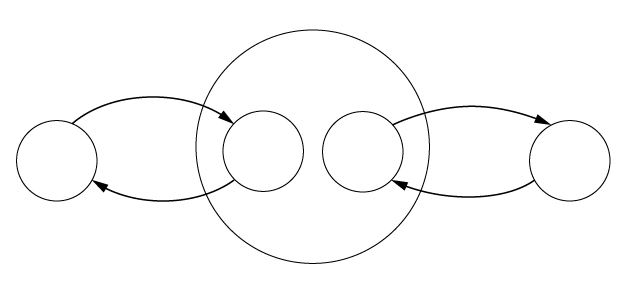
\includegraphics[scale=0.4]{introDiag}};
    \node (dv) at (-2.3, 0.0) {\huge $\dashv$};
    \node (IL) at (-3.58, -0.1) {IL};
    \node (vd) at (2.3, 0.0) {\huge $\dashv$};
    \node (coIL) at (3.65, -0.1) {coIL};

    \node (ILL) at (-0.67, 0.0) {ILL};
    \node (coILL) at (0.71, 0.0) {coILL};
    \node (BiILL) at (0, 1.0) {Bi-ILL};
  \end{tikzpicture}
    
\end{center}
The adjoint between IL and ILL is known as a LNL model of ILL, and is
due to Benton \cite{Benton:1994}.  However, the dual to LNL models
which would amount to the adjoint between coILL and coIL has yet to
appear in the literature.

Suppose $(\cat{I}, 1, \times, \to)$ is a cartesian closed category,
and $(\cat{L}, \top, \otimes, \limp)$ is a symmetric monoidal closed
category.  Then relate these two categories with a symmetric monoidal
adjunction $\cat{I} : \func{F} \dashv \func{G} : \cat{L}$
(Definition~\ref{def:SMCADJ}), where $\func{F}$ and $\func{G}$ are
symmetric monoidal functors.  The later point implies that there are
natural transformations $\m{X,Y} : \func{F}X \otimes \func{F}Y \mto
\func{F}(X \times Y)$ and $\n{A,B} : \func{G}A \times \func{G}B \mto
\func{G}(A \otimes B)$, and maps $\m\top : \top \mto \func{F}1$ and
$\n1 : 1 \mto \func{G}\top$ subject to several coherence conditions;
see Definition~\ref{def:SMCFUN}.  Furthermore, the functor $\func{F}$
is strong which means that $\m{X,Y}$ and $\m{\top}$ are isomorphisms.
This setup turns out to be one of the most beautiful models of
intuitionistic linear logic called a LNL model due to Benton
\cite{Benton:1994}.  In fact, the linear modality of-course can be
defined by $!A = \func{F}(\func{G}(A))$ which defines a symmetric
monoidal comonad using the adjunction; see Section~2.2 of
\cite{Benton:1994}.  This model is much simpler than other known
models, and resulted in a logic called LNL logic which supports mixing
intuitionistic logic with linear logic.  The main contribution of this
paper is the definition and study of the dual to Benton's LNL models
as models of cointuitionistic logic.

Taking the dual of the previous model results in what we call dual LNL
models. They consist of a cocartesian coclosed category, $(\cat{C}, 0,
+, -)$ where $- : \cat{C} \times \cat{C} \mto \cat{C}$ is left adjoint
to the coproduct, a symmetric monoidal coclosed category
(Definition~\ref{def:SMCCC}), $(\cat{L}', \perp, \oplus, \colimp)$,
where $\colimp : \cat{L}' \times \cat{L}' \mto \cat{L}'$ is left
adjoint to cotensor (sometimes called parr), and a symmetric
comonoidal adjunction (Definition~\ref{def:coSMCADJ}) $\cat{L'} :
\func{H} \dashv \func{J} : \cat{C}$, where $\func{H}$ and $\func{J}$
are symmetric comonoidal functors.  Similarly to above, this implies
that there are natural transformations $\m{X,Y} : \func{J}(X + Y) \mto
\func{J}X \oplus \func{J}Y$ and $\n{A,B} : \func{H}(A \oplus B) \mto
\func{H}A + \func{H}B$, and maps $\m0 : \func{J}0 \mto \perp$ and
$\n\perp : \func{H}\perp \mto 0$ subject to several coherence conditions;
see Definition~\ref{def:coSMCFUN}.  In fact, one can define Girard's
exponential why-not by $\wn A = \func{JH}A$, and hence, is the monad
induced by the adjunction.

Bellin \cite{Bellin:2012} was the first to propose the dual to
Bierman's \cite{Bierman:1994} linear categories which he names dual
linear categories as a model of cointuitionistic linear logic.  We
conduct a similar analysis to that of Benton for dual LNL models by
showing that dual LNL models are dual linear categories
(Section~\ref{subsec:dual_lnl_model_implies_dual_category}), and that
from a dual linear category we may obtain a dual LNL model
(Section~\ref{subsec:dual_category_implies_dual_lnl_model}).
Following this we give the definition of bi-LNL models by combining
our dual LNL models with Benton's LNL models to obtain a categorical
model of bi-intuitionistic logic
(Section~\ref{subsec:a_mixed_bi-linear_non-linear_model}), but we
leave its analysis and corresponding logic to a future paper.
Following the categorical model we define and analyze a new sequent
calculus (Section~\ref{sec:sequent_calculus}), natural deduction
formalization (Section~\ref{sec:sequent-style_natural_deduction}), and
a term assignment (Section~\ref{sec:term_assignment}) for dual LNL
logic.

***Introduce dual LNL logic.***

%%% Local Variables: 
%%% mode: latex
%%% TeX-master: main.tex
%%% End: 
